\chapter{CNNs for computer vision}
\label{image-ann}

A paper Visualizing and Understanding Convolutional Networks by Matthew D. 
Zeiler and Robert Fergus \cite{zf-net} started with two sentences: \textit{Large 
Convolutional Network models have recently demonstrated impressive 
classification performance on the~ImageNet benchmark. However there is no clear 
understanding of why they perform so well, or how they might be improved.}

I tried to disperse such clouds a bit in the~previous chapter, but now I would 
like to focus on another undertone connected with those statements. On their 
applications in the~computer vision.

Almost everything mentioned in chapter \ref{cnn} was already tied to
the~computer vision. The~following text will briefly describe the~field of computer 
vision itself and then introduce few tasks in that field connected with
the~topic of the~thesis. In each task, the~models that were considered during
the~research for the~practical part of this thesis - an implementation into GRASS 
GIS - will be mentioned. Models are also mentioned and described to depict their
evolution concluding in the~selected one.

% different sizes

\section{Understanding computer vision}
\label{computer-vision}

When you see a group photo, you can easily count the~number of people in
the~photo, you can say whether they are smiling or not, whether they are happy, sad, 
angry, you can even guess whether they are one family, a bunch of friends, 
colleagues or just random people passing by. You can do all of that in a 
fraction of a second without any effort. The~computer vision is supposed to be a 
computer-aided version of this human cognition. Or in a fancier way, from 
\cite{opencv}: \textit{Computer vision is the~transformation of data from a 
still or video camera into either a decision or a new representation.} the~new 
representation might be for instance a colour shift, the~decision an answer to a 
question like \textit{Is there any football field in the~picture?}

However, the~problem is that the~claim that it is easy for humans does not mean 
that it is easy also for computers. As is generally known and was indicated in 
chapter \ref{understanding-cnn}, the~human brain is an extremely complex tool. 
The other thing is that a computer receives a visual impulse (image) in another 
way as is illustrated in figure \ref{fig:mirror}. Where human sees a side 
mirror, a computer sees a grid of numbers. And this grid may be completely 
different when the~daytime, viewpoint, brightness, background or scale changes.

\begin{figure}[H]
   \centering
	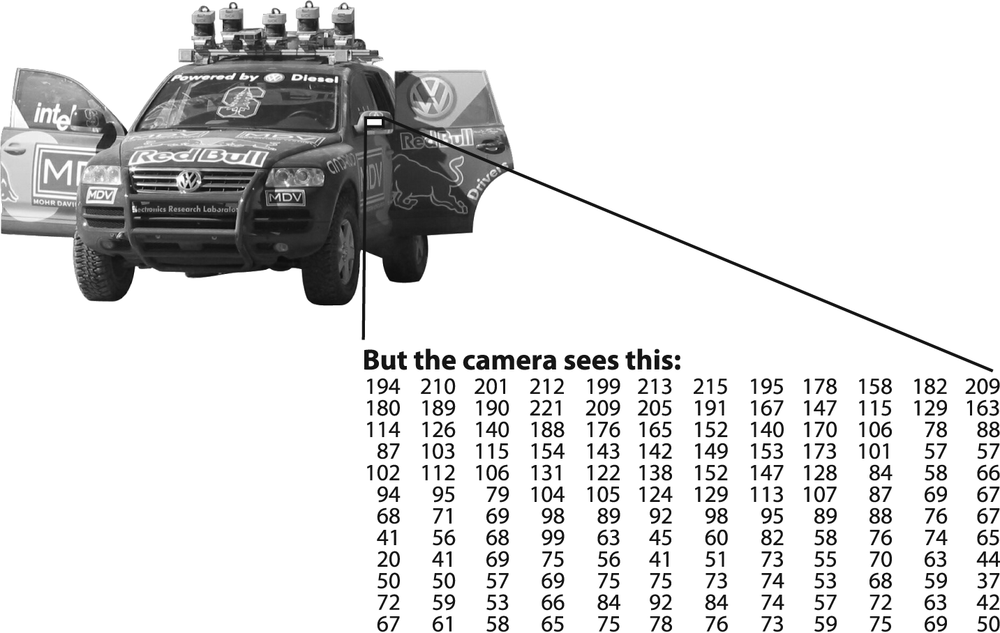
\includegraphics[width=.8\linewidth]{./pictures/comp-vision.png}
	\caption[Human and computer cognition]{The difference between human and 
computer cognition, source: \cite{opencv}}
      \label{fig:mirror}
\end{figure}

The task may be something like \textit{Is there any side mirror in the~picture?} 
This kind of tasks can be seen in the~field of computer vision daily and can be 
extremely difficult to solve in the~computer way. Although the~input may include 
some metadata, it still has to be solved in a strict mathematical way. And 
because our goal is to make our computer vision system \textit{perceive like a 
human}, it looks like the~right place for \zk{CNN}s.

Although we will focus only on classification and connected tasks like detection 
and segmentation, there are many more applications of the~computer vision. To 
name a few: Autonomous cars, face recognition, fingerprint recognition, motion 
capture, biometrics and remote sensing.

To get a better view into the~field of computer vision, it is recommended to 
read a richer source like \cite{comp-vision} and \cite{opencv} to get some 
practice.

\section{Classification}
\label{classification}

The idea is simple, image classification is the~task of assigning an image to 
one class. It means that the~user is interested in the~result of a guess of what 
the image contains. A good example is a camera trap. When the~user is interested 
in moose, he can train his model to predict moose and automatically filter all 
outputs from the~camera trap through this validator.

The idea of training a~model to sort a~list of numbers is quite 
straightforward. Due to differences in pictures of the~same object caused by 
influences mentioned in chapter \ref{computer-vision}, the~classification task 
needs a~bit of oblique, but still strictly logical thinking. It needs a 
data-driven approach. Instead of defining how exactly should moose look like, we 
feed the~model with a~bunch of labelled examples. It is the~same process as with 
human children.

However, the~number of classes does not have to be equal to one. The~user can 
have a~set of multiple classes and even his classifier may differ. A~popular 
simple classifier is a~binary classifier returning just 1 or 0 (representing 
True or False/Yes or no) for each class per image but much more widely used one 
is a~softmax function giving a~vector of probabilities for classes. This 
classifier also somehow more represents the~human mind, as we may be unsure if 
there is a~moose or a~wapiti in the~picture if it was taken with bad 
conditions.

\begin{figure}[H]
   \centering
	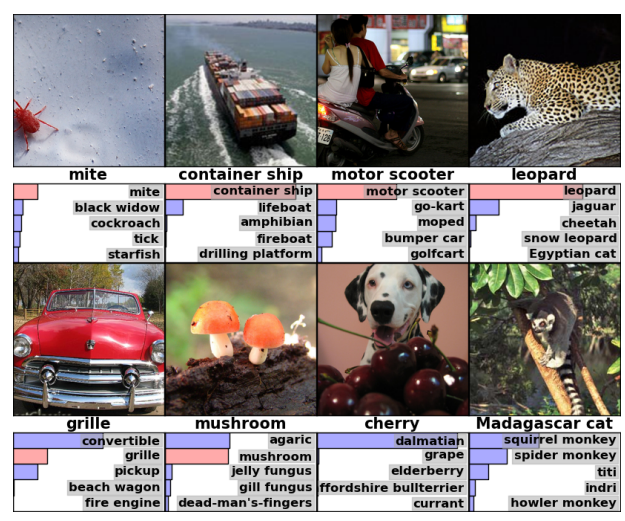
\includegraphics[width=.8\linewidth]{./pictures/classification.png}
	\caption[Classification example]{An example of the~classification output with 
softmax function, source: \cite{cnn-classification}}
      \label{fig:class}
\end{figure}

The pioneering work in the~field of \zk{CNN}-based classification is AlexNet 
proposed in \cite{cnn-classification} and described in chapter \ref{alexnet}. 
Another interesting implementation is the~CNN-RNN framework for multi-label 
image classification\footnote{Real world images often contain more features; 
multi-label image classification tries to predict more than just one of them. 
The problem of one-label classification can be seen in the~seventh image in 
figure \ref{fig:class}.} proposed in \cite{multi-classification}.

\section{Classification with localization}
\label{classification-localization}

Although classification with localization is sometimes ignored in similar lists 
as a~subtype of object detection, I believe it is useful to mention it as a~step 
between pure classification and object detection.

Classification was already explained in the~previous chapter. Classification 
with localization uses classification in its one-class form together with 
bounding boxes (bounding boxes may be multiple). the~goal is to draw
the~bounding box as tight around the~object as possible and predict the~class of
the~object, so the~user ends up with two outputs:
\begin{itemize}
	\item \textbf{Class:} Class label
	\item \textbf{Bounding box:} Box in the~image defined by two coordinates and 
its width and height.
\end{itemize}

Because multiple values are returned, this task can be considered as a~kind of
a~regression problem. Outputs from the~regression are enough to get a~result as 
the one illustrated in figure \ref{fig:class-loc}. 

\begin{figure}[H]
   \centering
	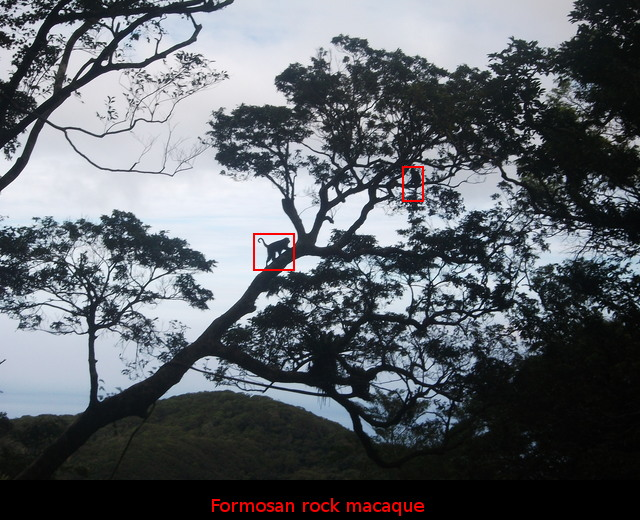
\includegraphics[width=.7\linewidth]{./pictures/class-loc.JPG}
	\caption[Classification with localization example]{An example of classification 
with localization}
      \label{fig:class-loc}
\end{figure}

\section{Object detection}
\label{object-detection}

Object detection is the~classification with localization for multiple classes.

Shared basics with the~task from the~previous chapter instigate to use
the~similar approach but applied to every single class individually. However, this 
method could be very, very inefficient. Different architectures use different 
practice to solve it and few of them will be presented here.

\subsection{R-CNN}
\label{r-cnn}

The Region-based convolutional neural network (\zk{R-CNN}) is a~model proposed 
in 2014 in \cite{rcnn}, which combines region proposals with convolutional 
neural networks to detect objects in an image via bounding boxes. 

The first step of the~detection and also an answer to individual passes of 
classes is to generate category-independent region proposals containing probable 
objects. Instead of the~whole image, those proposals are passed to a~deep 
convolutional neural network which returns a~feature vector for each region 
proposal. The~last step is to pass this vector through a~set of class-specific 
linear support vector machines (\zk{SVM}s).

Although diverse methods may be used for the~region proposals 
generation\footnote{In the~case of interest see an \textit{objectness measure} 
\cite{objectness} or \textit{category-independent object proposals with diverse 
ranking} \cite{cat-independent-proposals}.}, authors of the~original R-CNN paper 
decided to use the~selective search. The~selective search was proposed in 
\cite{selective-search} and mixes advantages of both an exhaustive search and 
segmentation. From the~exhaustive search, an effort to catch all possible object 
locations is used; from segmentation, the~idea of following the~image structure 
to guide the~sampling process is used. To deal with many diverse image 
conditions, the~selective search uses a~variety of complementary image 
partitions.

After regions proposition, their features must be computed. Because the~network 
works with a~fixed-size input, the~region must be warped into $227 \times 227$ 
square RGB image, and then it can be forward propagated through an architecture 
composed of five convolutional layers and two fully connected layers (a modified 
architecture of AlexNet, see chapter \ref{alexnet}).

The third step is scoring those extracted features (deciding which class
the~feature is and whether it is any class at all). This is done for each feature 
separately using an \zk{SVM} trained for that class.

In general, the~bounding box has a~large overlap with the~background. This is 
the last problem with which the~algorithm has to deal. To improve
the~localization (make bounding boxes tighter), a~linear bounding box regression 
method proposed in \cite{object-det} is used with one modification - R-CNN 
applies regression on features computed by the~CNN instead of on geometric 
features computed on the~inferred deformable part model (\zk{DPM}) locations.

\begin{figure}[H]
   \centering
	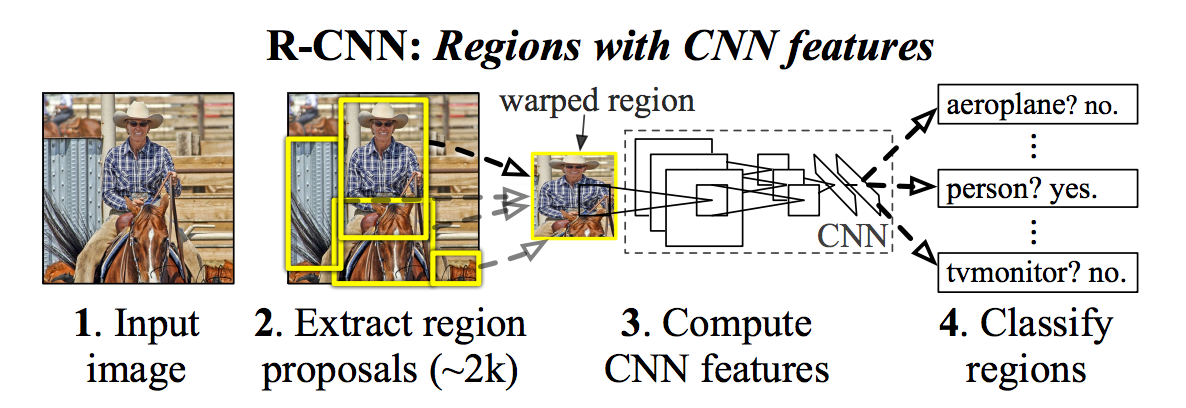
\includegraphics[width=.9\linewidth]{./pictures/rcnn.png}
	\caption[R-CNN architecture]{R-CNN architecture schema, source: \cite{rcnn}}
      \label{fig:rcnn}
\end{figure}

Although R-CNN outperformed similar architectures\footnote{\cite{rcnn} claims
a~mean average precision (\zk{mAP}) of $53.3 \%$.}, there were still some 
shortcomings. The~biggest one was the~slowness caused mainly by three elements - 
the forward propagation through \zk{CNN} (each region of every image must be 
passed separately), by its triplicated training (a network for generating image 
features, a~network for the~class decision and the~bounding box regression 
model) and by the~generating of bounding box proposals.

\subsection{Fast R-CNN}
\label{fast-rcnn}

Then, in the~year 2015, a~new architecture came to solve first two of these issues. 
Because the~main reason for a~new architecture was to speed-up \zk{R-CNN}, Ross 
Girshick named his new architecture proposed in \cite{fast-rcnn} simply Fast 
\zk{R-CNN}. Besides the~main purpose to avoid first two issues mentioned in 
chapter \ref{r-cnn}, it also improves its accuracy\footnote{\cite{fast-rcnn} 
claims a~\zk{mAP} of $66 \%$ on Pascal Visual object classes (\zk{VOC}) 2012. To 
find more info about the~Pascal \zk{VOC} datasets and challenges, please see 
\cite{voc}.}.

The first issue, the~separate forward propagation for each region proposal, was 
solved by propagating the~entire image to obtain a~feature map before the~region 
proposition. For each object proposal is from the~feature map extracted
a~fixed-length feature vector by a~region of interest (\zk{RoI}) pooling layer.

The \zk{RoI} pooling layer can be seen as an one-level spatial pyramid pooling 
layer, a~max pooling-based downsampling algorithm proposed in \cite{spp}. Its 
purpose is to decompose separately each valid \zk{RoI} into a~fixed size $7 
\times 7$ feature map. The~decomposition is made by quantization each \zk{RoI} 
to the~rounded discrete grid which is filled using max pooling on
the~corresponding kernel of the~feature map.

These feature vectors are inputs for a~set of \zk{FC} layers. This propagation 
is followed by the~last, branched step, where two different outputs are obtained 
depending on the~last layer - class probabilities from a~softmax function and
a~bounding box defined by 4 values from a~regressor.

There can be seen also a~solution to the~second problem named in chapter 
\ref{r-cnn}. Instead of three separate models, all steps are joint into only one 
model by appending classification (using a~softmax layer instead of a~separate 
\zk{SVM}) and bounding box regression as parallel layers to the~end of
the~model.

\begin{figure}[H]
   \centering
	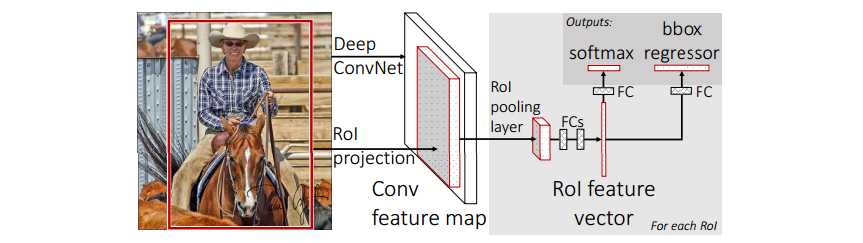
\includegraphics[width=.9\linewidth]{./pictures/fastrcnn.png}
	\caption[Fast R-CNN architecture]{Fast R-CNN architecture schema, source: 
\cite{fast-rcnn}}
      \label{fig:fast-rcnn}
\end{figure}

There can be raised a~question whether is the~\zk{SVM} replacement with
the~softmax layer as accurate as the~original approach. According to tests performed 
in \cite{fast-rcnn}, the~softmax layer is even slightly outperforming \zk{SVM} 
by 0.1 to 0.8 \zk{mAP} points depending on the~depth of
the~network\footnote{Different models were tried. Surprisingly, with a~deeper network, 
smaller \zk{mAP} difference was noticed.}.

\subsection{Faster R-CNN}
\label{faster-rcnn}

The third speed issue mentioned in chapter \ref{r-cnn}, the~region proposer 
based on the~selective search, was solved in the~year 2016 in an architecture 
imaginatively named Faster \zk{R-CNN}, proposed in \cite{faster-rcnn}.

Microsoft Research team found that the~feature map computed in the~first part of 
Fast \zk{R-CNN} can be used to generate region proposals instead of using slower 
selective search algorithm. Authors did it by including Region Proposal 
Network \zk{RPN} after the~feature maps extraction of Fast R-CNN.

\begin{figure}[H]
   \centering
	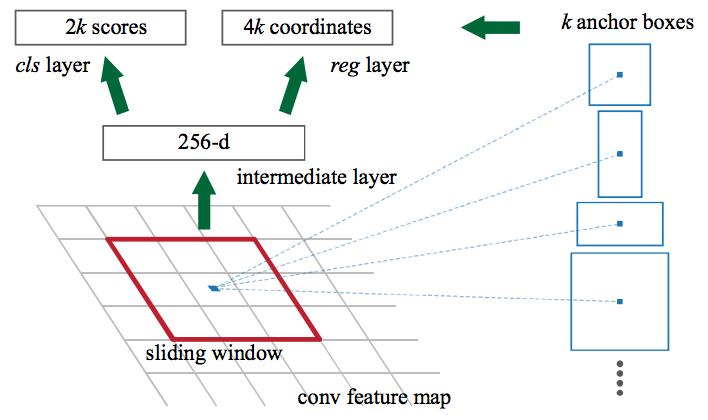
\includegraphics[width=.5\linewidth]{./pictures/fasterrcnn-anchors.png}
	\caption[Region proposal network]{\zk{RPN} schema, source: \cite{faster-rcnn}}
      \label{fig:rpn}
\end{figure}

\zk{RPN} approach is different than the~ones used in other architectures. 
Instead of pyramids of images or filters, \zk{RPN} uses anchor boxes - a~set of 
rectangular bounding boxes proposals and scores created by sliding a~spatial 
window over the~entire feature map. The~sliding window is a~$n \times n$ fully 
convolutional network. The~anchor boxes are defined by a~scale and aspect ratio, 
so they are of different shapes. Powerful attributes of anchor boxes are that 
they are translation-invariant and multi-scale, which concludes also into
a~reduction of the~model size.

\begin{figure}[H]
   \centering
	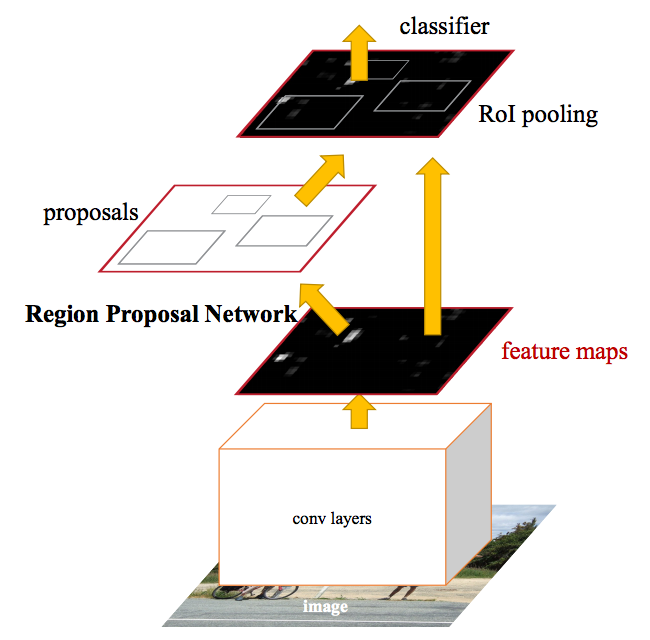
\includegraphics[width=.55\linewidth]{./pictures/fasterrcnn.png}
	\caption[Faster R-CNN architecture]{Faster \zk{R-CNN} architecture schema, 
source: \cite{faster-rcnn}}
      \label{fig:faster-rcnn}
\end{figure}

As can be seen in figure \ref{fig:faster-rcnn}, the~training scheme alternates 
between training (or fine-tuning) for the~region proposition and for object 
detection. This approach with shared convolutional features quickly converges.

Besides the~speed improvement, Faster \zk{R-CNN} improves also the~accuracy. 
\cite{faster-rcnn} claims a~\zk{mAP} of $73.2 \%$ on Pascal \zk{VOC} 2007 and of 
$70.4 \%$ on Pascal \zk{VOC} 2012.

% TODO: Single-Shot MultiBox Detector (SSD) You Only Look Once (YOLO)

\section{Semantic segmentation}
\label{semantic-segmentation}

Semantic segmentation is a~labelling of each pixel in an image to a~certain 
class without differentiating between instances of objects.

The first conception in our minds is to slide the~kernel across an entire image 
and classify each pixel individually. However, I think that everyone surmises 
that this conception is not very efficient.

Two terms are connected with semantic segmentation, \textit{encoder} and 
\textit{decoder}. While the~encoder is a~classification network as one of those 
described in chapter \ref{cnn-architectures}, the~decoder is a~network 
projecting a~lower resolution (a feature map) to a~higher one (pixel space of 
the original image size), e.g. The~task of the~decoder is to recover the~spatial 
information lost in the~encoder. Different versions of decoders were proposed.

\subsection{Fully convolutional network}
\label{fcns}

The Fully convolutional network (\zk{FCN}) was proposed by Jonathan Long and
the~UC Berkeley team in 2015 in \cite{fcns}.

\begin{figure}[H]
   \centering
	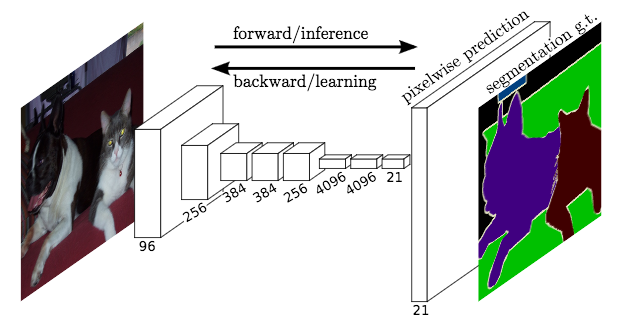
\includegraphics[width=.8\linewidth]{./pictures/fcns.png}
	\caption[Fully convolutional network]{Semantic segmentation with \zk{FCN} 
schema, source: \cite{fcns}}
      \label{fig:fcns}
\end{figure}

Imagine for example VGG-16 as the~backbone architecture, but the~same process 
can be applied to any other classification architecture. Following the~approach 
of \cite{fcns}, cut off the~last classification layer and convert the~fully 
connected layers into convolutional ones. $1 \times 1$ convolution was appended 
to predict scores for each class. 

Everything must be then passed through the~decoder; the~decoder is here 
represented by a~backward convolution, by a~\textit{deconvolution}. 
Deconvolution consists of upsampling using a~bilinear interpolation. With a~few 
of deconvolutional layers, the~network can learn even a~nonlinear upsampling. 
When using more layers, it is useful to fuse the~output of each layer with 
predictions computed in the~backbone layer with corresponding resolution using 
similar bypass (skip connections) as that described in chapter \ref{resnet}.

\begin{figure}[H]
   \centering
	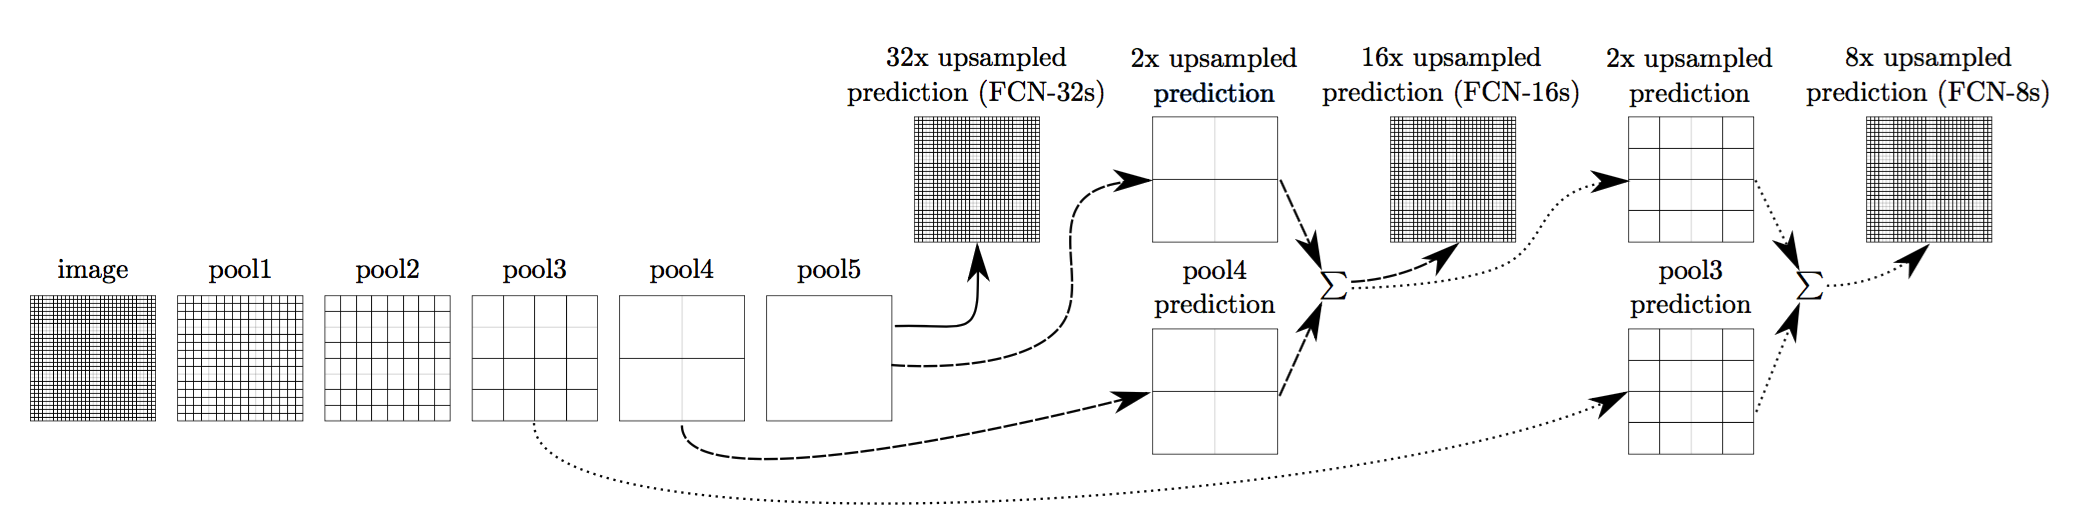
\includegraphics[width=\linewidth]{./pictures/fcns-bypass.png}
	\caption[Bypass in Fully convolutional network]{\zk{FCN} skip connections 
schema; only pooling and prediction layers are shown, source: \cite{fcns}}
      \label{fig:fcns-bypass}
\end{figure}

% segnet, fully convolutional densenet 

\section{Instance segmentation}
\label{instance-segmentation}

Instance segmentation can be seen as a~combination of object detection and 
semantic segmentation; the~task is in detecting all instances of different 
objects and marking their pixels. In other words, the~difference between 
semantic segmentation and instance segmentation is that instance segmentation 
allows marking two objects of the~same class separately.

\begin{figure}[H]
   \centering
	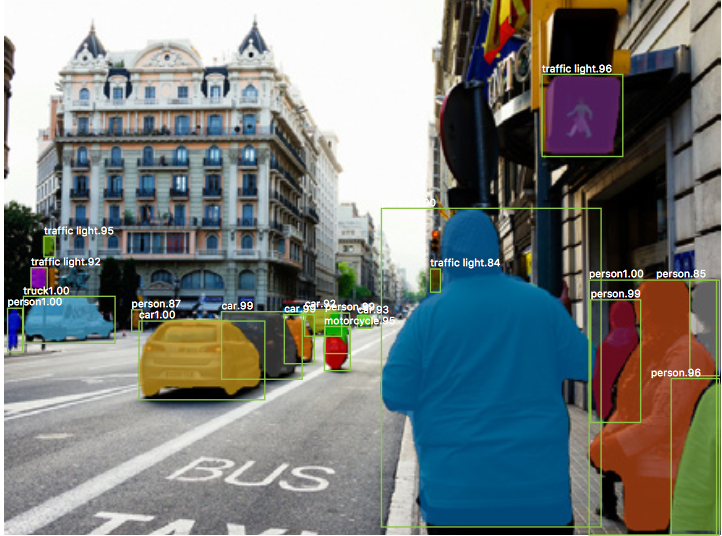
\includegraphics[width=0.8\linewidth]{./pictures/instance-segmentation.png}
	\caption[Instance segmentation example]{Instance segmentation example, source: 
\cite{mask-rcnn}}
      \label{fig:instance-segmentation}
\end{figure}

\subsection{Mask R-CNN}
\label{mask-rcnn}

So we had \zk{R-CNN}, Fast \zk{R-CNN} and Faster \zk{R-CNN}. What could be
the~next step? The~first answer that comes to your mind is wrong - instead of 
expected \textit{The Fastest \zk{R-CNN}}, the~Mask \zk{R-CNN} was proposed in 
the year 2017 by Facebook AI Research \zk{FAIR} in \cite{mask-rcnn}.

\zk{FAIR} stood in a~front of another question. According to \cite{faster-rcnn}, 
Faster R-CNN outperformed most of their competitors in the~field of object 
detection. But it was still unusable for some users looking for a~semantic 
segmentation neural network. They had a~powerful network for object detection, 
so the~question was: Is there any way to use the~current network for
the~semantic segmentation?

Obviously, the~answer was \textit{yes}. But instead of the~semantic 
segmentation, they proposed a~more advanced approach, the~instance segmentation. 
To implement the~instance segmentation with sufficient accuracy, there was
a~need for some changes in the~architecture of Faster \zk{R-CNN}. Following
the~original terminology from \cite{mask-rcnn}, in the~following part, I will 
distinguish between the~backbone architecture for feature extraction and
the~head architecture for classification, bounding box regression and mask 
prediction. Those will be described in following parts of this chapter along 
with an extra focus on a~RoIAlign, a~new approach in the~\zk{RoI} generation.

\begin{figure}[H]
   \centering
	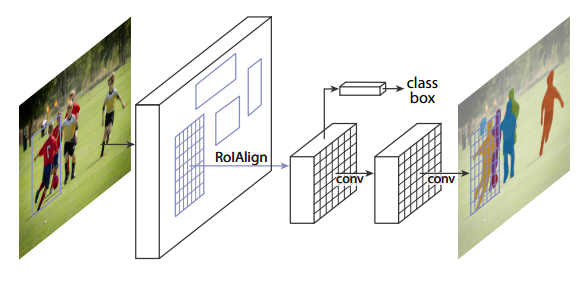
\includegraphics[width=0.4\linewidth]{./pictures/maskrcnn.png}
	\caption[Mask R-CNN architecture]{Mask \zk{R-CNN} architecture schema, source: 
\cite{mask-rcnn}}
      \label{fig:mask-rcnn}
\end{figure}

\subsubsection{Backbone architecture}
\label{backbone}

For the~backbone architecture, more models can be used, but in the~original 
paper \cite{mask-rcnn}, ResNet was used. ResNet was already described in chapter 
\ref{resnet}.

Moreover, authors experimented also with ResNet extended by a~feature pyramid 
network (\zk{FPN}), a~top-down architecture with skip connections (in
the~original paper called \textit{lateral connections}) developed for building 
high-level semantic feature maps at different scales proposed in \cite{fpn}.

\zk{FPN} uses the~fact that by subsampling, we obtain a~different spatial 
resolution feature hierarchy with multi-scale, pyramidal shape. To achieve 
strong semantics at all scales, \zk{FPN} uses bottom-up, top-down pathways and 
skip connections to create predictions independently on each pyramid level.
The~feature hierarchy is created by propagating an image through the~convolutional 
network (bottom-up pathway). There are stacks of layers producing feature maps 
of the~same size; they are thought of being in the~same stage. One level of
the~\zk{FPN} is created from the~output of the~last layer of each stage except
the~first stage due to its memory claims. The~top-down pathway is done by upsampling 
feature maps from higher levels by a~factor of 2 and using nearest neighbour 
upsampling, and then enhancing them via skip connections with features from
the~bottom-up pathway as can be seen in figure \ref{fig:fpn}.

\begin{figure}[H]
   \centering
	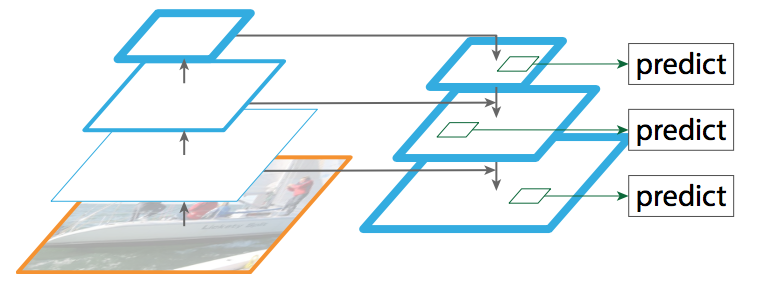
\includegraphics[width=0.4\linewidth]{./pictures/top-down.png}
	\caption[Feature pyramid network]{The \zk{FPN} schema, source: \cite{fpn}}
      \label{fig:fpn}
\end{figure}

\subsubsection{Head architecture}
\label{head}

In the~head architecture, there was the~most important change to allow
the~instance segmentation - including the~mask branch in parallel with branches for 
classification and bounding box regression. 

The mask branch is a~pixel-to-pixel \zk{FCN} predicting a~mask individually for 
each \zk{RoI}, where the~mask is a~binary matrix of ones (object location) and zeros 
(elsewhere).

In figure \ref{fig:head}, we can see two implementations of the~head 
architecture. The~left one is based on ResNet-C4 (4 stage ResNet) and extends it 
with the~compute-intensive fifth stage, the~right one is based on \zk{FPN} which 
already includes the~fifth stage. In these implementations, the~last convolution 
is $1 \times 1$ and the~other ones are $3 \times 3$ and are the~ones with 
preserved shapes; deconvolutions are $2 \times 2$ with stride 2 and increase 
shapes. 

\begin{figure}[H]
   \centering
	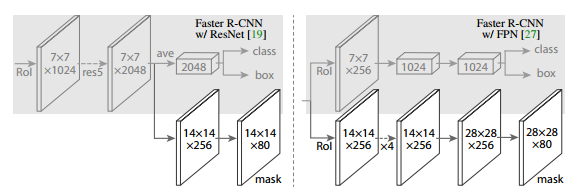
\includegraphics[width=0.7\linewidth]{./pictures/maskrcnn-head.png}
	\caption[Mask R-CNN head architecture]{Different Mask \zk{R-CNN} head 
architectures schema, source: \cite{mask-rcnn}}
      \label{fig:head}
\end{figure}

\subsubsection{RoIAlign}
\label{roialign}

In figure \ref{fig:mask-rcnn}, we can see a~RoIAlign layer instead of Fast 
\zk{R-CNN} \zk{RoI} pooling from figure \ref{fig:fast-rcnn}.

This change was needed because of spatial inaccuracy of \zk{RoI} pooling due to 
the fact that it was not intended to be used for a~pixel-to-pixel alignment. 
This inaccuracy is caused by quantizations and roundings and RoIAlign avoids it 
simply by skipping the~rounding. To compute the~value of the~input, a~bilinear 
interpolation at regular sampled locations (usually 4) is used.

According to \cite{mask-rcnn}, RoiAlign improved Mask R-CNN mask accuracy by 
relative 10 \% to 50 \%.

% \section{Content-based Image Retrieval}
